Le cours a porté sur deux outils très utiles en géométrie : le théorème du pôle Sud et la puissance d'un point par rapport à un cercle.


\subsubsection{Exercices}


\begin{exo}
Soient $k_1$ et $k_2$ deux cercles s'intersectant en deux points distincts $A$ et $B$. Une tangente $t$ commune aux deux cercles touche le cercle $k_1$ en un point $C$ et le cercle $k_2$ en un point $D$. Soit $M$ le point d'intersection de la droite $(AB)$ avec la tangente $t$. Montrer que $M$ est le milieu du segment $[CD]$.
\end{exo}


\begin{exo}
Soit $ABC$ un triangle et $D$ le pied de la bissectrice issue de $B$. Les cercles circonscrits aux triangles $ABD$ et $BCD$ recoupent les côtés $[AB]$ et $[BC]$ en $E$ et $F$ respectivement. Montrer que $AE=CF$.
\end{exo}


\begin{exo}
Soit $ABC$ un triangle acutangle. La hauteur issue de $B$ dans $ABC$ intersecte le cercle de
diamètre $[AC]$ en $K$ et $L$, et la hauteur issue de $C$ dans $ABC$ intersecte le cercle de diamètre $[AB]$ en $M$ et $N$. Montrer que $K$, $L$, $M$ et $N$ sont cocycliques.
\end{exo}


\begin{exo}
Soit $ABCD$ un quadrilatère cyclique. On appelle respectivement $I_A$, $I_B$, $I_C$ et $I_D$ les centres des cercles inscrits des triangles $BCD$, $DCA$, $ADB$ et $BAC$. Quelle est la nature du quadrilatère $I_AI_BI_CI_D$ ?
\end{exo}


\begin{exo}
Soit $ABC$ un triangle aux angles aigus avec $AC<AB$ et soit $k$ son cercle circonscrit. La tangente au cercle $k$ en $A$ intersecte $(BC)$ en un point $P$. Soit $M$ le milieu du segment $[PA]$ et soit $R$ le second point d'intersection de la droite $(MB)$ avec le cercle $k$. La droite $(PR)$ recoupe $k$ en un point $S$. Montrer que les droites $(CS)$ et $(AP)$ sont parallèles.
\end{exo}


\begin{exo}
Soient $ABC$ un triangle et $D$ l'intersection de la bissectrice intérieure issue de $A$ avec $[BC]$. La médiatrice de $[AD]$ recoupe la bissectrice issue de $B$ en $M$ et celle issue de $C$ en $N$. Montrer que les points $A$, $I$, $M$ et $N$ sont sur un même cercle.
\end{exo}


\begin{exo}
Soient $A$, $B$, $C$ et $D$ quatre points fixés sur un cercle. Quelle est la courbe décrite par l'ensemble des points $X$ tels que les cercles circonscrits aux triangles $XAB$ et $XCD$ sont tangents en $X$ ?
\end{exo}


\subsubsection{Solutions}


\begin{sol}
Calculons la puissance du point $M$ par rapport à chacun des deux cercles en utilisant la définition de $M$ et la tangence de la droite $t$ :
\begin{gather*}
    \mathcal{P}_{k_1}(M) = MA \cdot MB = MC^2, \\
    \mathcal{P}_{k_2}(M) = MA \cdot MB = MD^2.
\end{gather*}
Ainsi, $\mathcal{P}_{k_1}(M) = \mathcal{P}_{k_2}(M) = MA \cdot MB$. On en déduit que $MC^2 = MD^2$, ce qui prouve que $M$ est le milieu de $[CD]$.
\end{sol}


\begin{sol}
\textbf{Première solution.} D'après le théorème du pôle Sud appliqué dans les triangles $ABF$ et $CBE$, nous savons que d'une part $DA=DF$ et d'autre part que $DE=DC$. Qui plus est, le théorème de l'angle inscrit donne $\widehat{CBE}=\widehat{EDA}$ (cocyclicité de $B$, $C$, $D$ et $E$) et $\widehat{ABF}=\widehat{FDC}$ (cocyclicité de $A$, $B$, $F$, $D$). Ainsi, $\widehat{ADE}=\widehat{FDC}$. Mis avec les égalités de longueurs précédentes, on en conclut que les triangles $ADE$ et $FDC$ sont superposables, ce qui implique que $AE=CF$.

\begin{figure}[!h]
\centerline{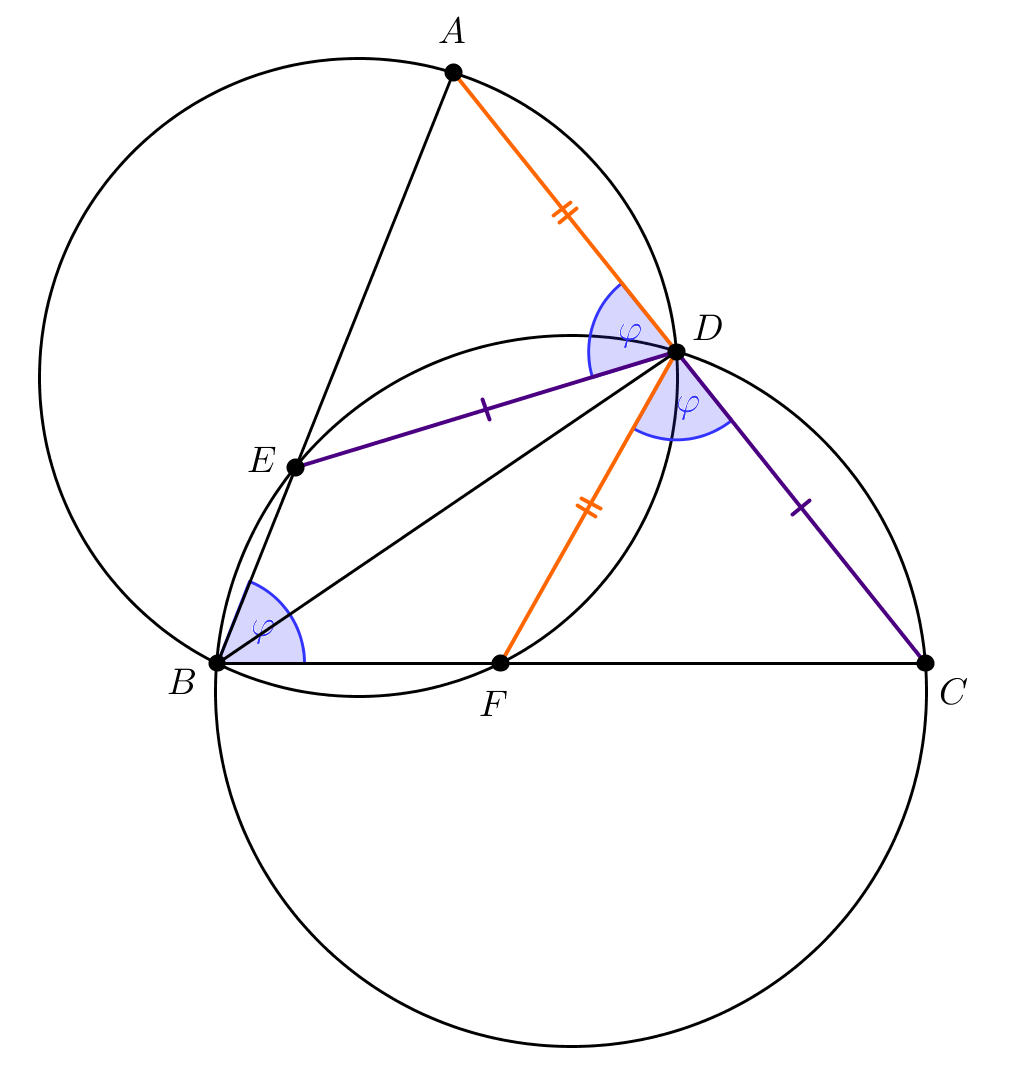
\includegraphics[width=0.35\textwidth]{pied_bissectrice}}
\end{figure}

\textbf{Seconde solution.} Comme ce qu'on cherche à prouver ne semble pas traduire de propriété angulaire intéressante, une approche métrique semble plus appropriée. Écrivons donc les puissances des points $A$ et $C$ par rapport aux cercles circonscrits à $BDC$ et $ADB$ respectivement :
\[ AE.AB = AD.AC \text{\ \ \ et\ \ \ } CA.CD = CF.CB \]
En faisant le quotient de ces deux relations, il vient $\frac{AD}{CD} = \frac{AB}{BC}.\frac{AE}{CF}$. Or, d'après le théorème de la bissectrice, $\frac{AD}{CD} = \frac{AB}{BC}$, d'où $\frac{AE}{CF}=1$, ce qui donne le résultat escompté.
\end{sol}


\begin{sol}
Tout d'abord, on remarque que le cercle $\Gamma_B$ de diamètre $[AC]$ passe par les pieds des hauteurs issues de $A$ et de $C$. De même, le cercle $\Gamma_C$ de diamètre $[AB]$ passe par les pieds des hauteurs issues de $A$ et $B$. Notons $H_A$ le pied de la hauteur issue de $A$ et $H$ l'orthocentre du triangle $ABC$.

En écrivant la puissance de l'orthocentre par rapport à chacun des deux cercles, il vient
\begin{gather*}
    \mathcal{P}_{\Gamma_B}(H) = HL \cdot HK = HA \cdot HH_A, \\
    \mathcal{P}_{\Gamma_C}(H) = HM \cdot HN = HA \cdot HH_A.
\end{gather*}
Dès lors, $\mathcal{P}_{\Gamma_B}(H) = \mathcal{P}_{\Gamma_C}(H) = HA \cdot HH_A$. Par conséquent, on a $HL \cdot HK = HM \cdot HN$, ce qui prouve que $K$, $L$, $M$ et $N$ sont cocycliques.
\end{sol}


\begin{sol}
Il s'agit d'utiliser le théorème du pôle Sud pour faire apparaître des points cocycliques puis de conclure par chasse aux angles. Appelons $S$ le milieu de l'arc $\wideparen{AB}$. $I_C$ étant le centre du cercle inscrit de $DAB$, le théorème du pôle Sud nous dit que $SA=SB=SI_C$. De même, $SA=SB=SI_D$. Finalement, c'est que $A$, $B$, $I_C$ et $I_D$ sont cocycliques, et on montre de même que les quadrilatères $BCI_AI_D$, $CDI_BI_A$ et $DAI_CI_B$ sont cycliques. On en tire :

\begin{align*}
(I_AI_D,I_AI_B) &= (I_AC,I_AI_B)+(I_AI_D,I_AC) \text{\ \ d'après la relation de Chasles}\\
&= (DI_B,DC)+(BI_D,BC) \text{\ \ car les quadrilatères $CDI_BI_A$ et $BCI_AI_D$ sont cycliques}\\
&= \frac{(DA,DC)}{2}+\frac{(BA,BC)}{2} \text{\ \ par définition des points $I_B$ et $I_D$}\\
&= 90 \text{\ \ car $A$, $B$, $C$ et $D$ sont cocycliques, soit $(DA,DC)+(BA,BC)=180$}
\end{align*}
En faisant de même autour des points $I_B$, $I_C$ et $I_D$, on en conclut qu'$I_AI_BI_CI_D$ est un rectangle.

\begin{figure}[!h]
\centerline{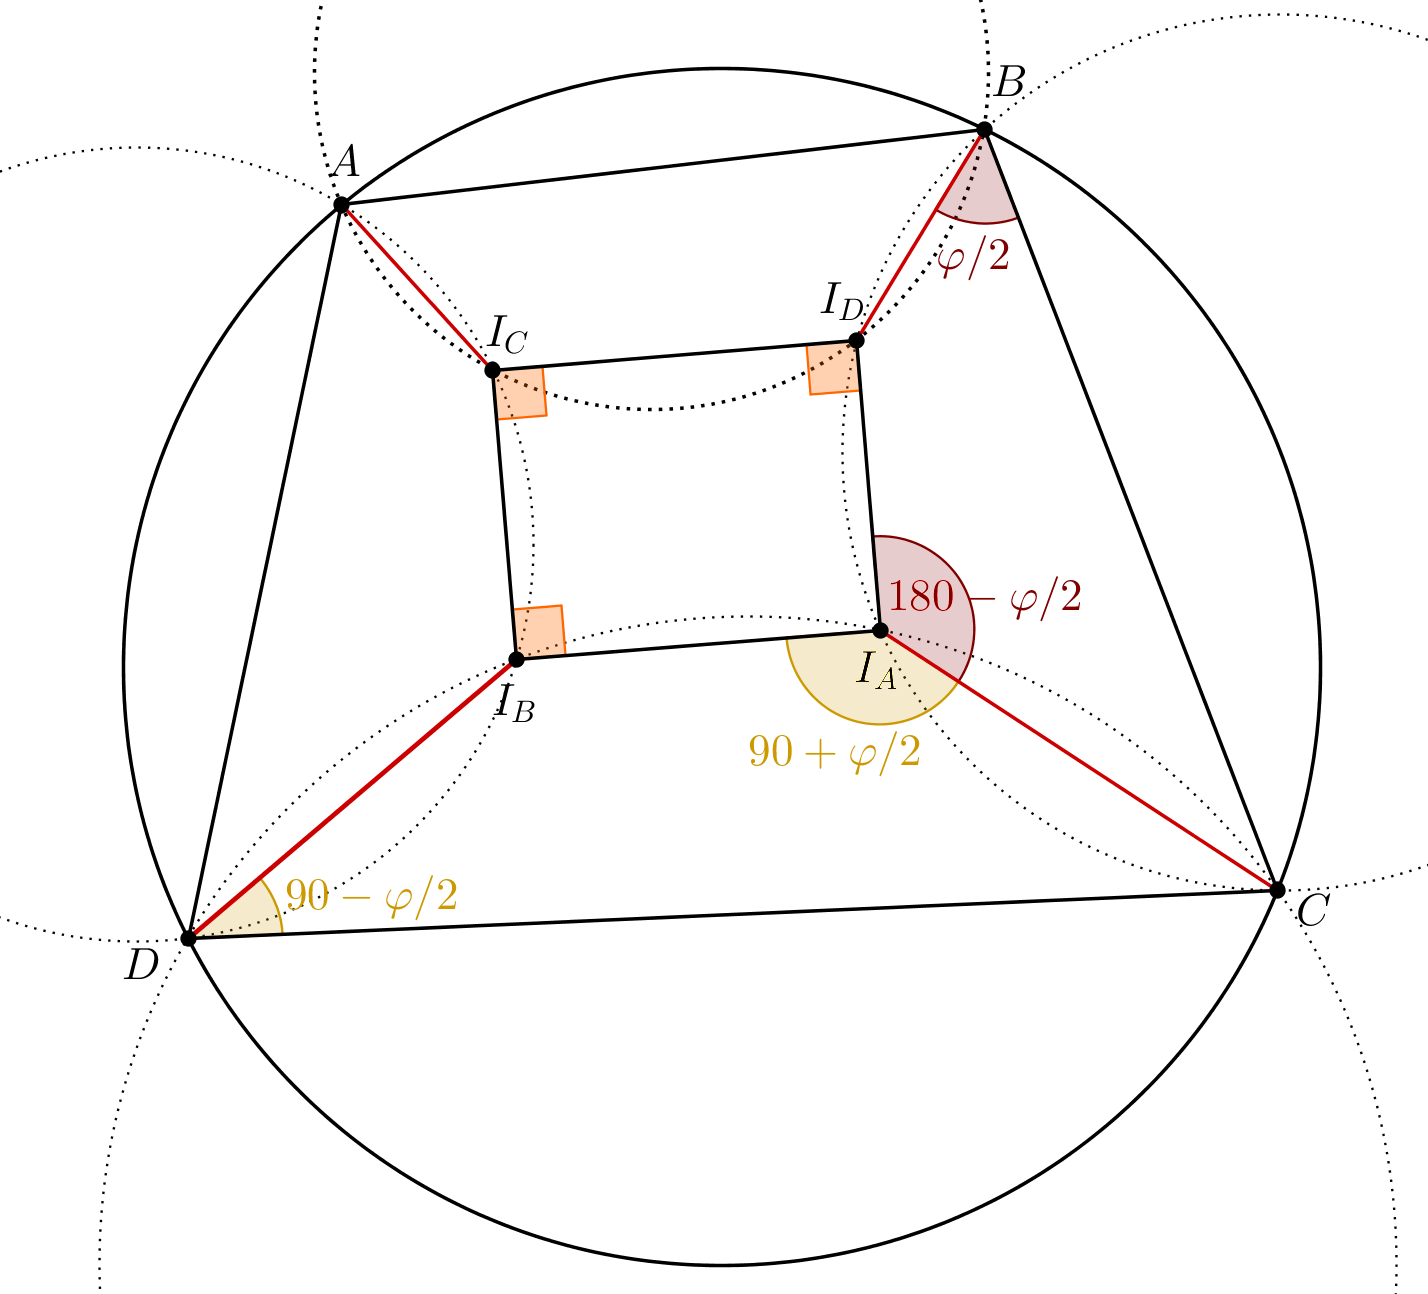
\includegraphics[width=0.5\textwidth]{rectangle_X}}
\end{figure}
\end{sol}


\begin{sol}
Par la puissance du point $M$ par rapport au cercle $k$, $MA^2=MR\cdot MB$. Puisque $M$ est le milieu du segment $[AP]$, $MP^2=MA^2=MR\cdot MB$. Par la réciproque de la puissance d'un point, la droite $(MP)$ est tangente au cercle circonscrit au triangle $PRB$. Il vient $\widehat{MPS}=\widehat{MPR}=\widehat{PBR}$ et puisque les points $R,C,B$ et $S$ sont cocycliques, $\widehat{CBR}=\widehat{CSR}$ donc $\widehat{APS}=\widehat{PSC}$.

\definecolor{qqwuqq}{rgb}{0.0,0.39215686274509803,0.0}
\definecolor{uuuuuu}{rgb}{0.26666666666666666,0.26666666666666666,0.26666666666666666}
\definecolor{ffqqqq}{rgb}{1.0,0.0,0.0}
\definecolor{uququq}{rgb}{0.25098039215686274,0.25098039215686274,0.25098039215686274}
\begin{center}
\begin{tikzpicture}[line cap=round,line join=round,>=triangle 45,x=1.0cm,y=1.0cm]
\clip(-4.92,-4.880000000000003) rectangle (18.080000000000002,6.200000000000001);
\draw [shift={(-4.166666666666667,-3.0)},color=qqwuqq,fill=qqwuqq,fill opacity=0.1] (0,0) -- (24.11022907079737:0.6) arc (24.11022907079737:39.936383146969916:0.6) -- cycle;
\draw [shift={(10.0,-3.0)},color=qqwuqq,fill=qqwuqq,fill opacity=0.1] (0,0) -- (164.17384592382746:0.6) arc (164.17384592382746:180.0:0.6) -- cycle;
\draw [shift={(9.082352941176472,2.9294117647058826)},color=qqwuqq,fill=qqwuqq,fill opacity=0.1] (0,0) -- (-155.88977092920265:0.6) arc (-155.88977092920265:-140.06361685303008:0.6) -- cycle;
\draw(6.0,-0.5833333333333334) circle (4.6733582976033174cm);
\draw [color=ffqqqq,domain=-4.92:18.080000000000002] plot(\x,{(--1.75--3.0*\x)/3.5833333333333335});
\draw [domain=-4.92:18.080000000000002] plot(\x,{(--24.0-0.0*\x)/-8.0});
\draw [domain=-4.92:18.080000000000002] plot(\x,{(--1.7500000000000004--3.0*\x)/-10.583333333333334});
\draw [domain=-4.92:18.080000000000002] plot(\x,{(-6.236585365853658--2.4585365853658536*\x)/5.49349593495935});
\draw [color=ffqqqq] (9.082352941176472,2.9294117647058826)-- (2.0,-3.0);
\draw (2.0,-3.0)-- (3.0,3.0);
\draw (3.0,3.0)-- (10.0,-3.0);
\draw (10.0,-3.0)-- (2.0,-3.0);
\draw [dotted] (2.916666666666667,-11.460648148148149) circle (11.0343182026745cm);
\begin{scriptsize}
\draw [fill=uququq] (3.0,3.0) circle (1.5pt);
\draw[color=uququq] (2.88,3.2800000000000002) node {$A$};
\draw [fill=uququq] (10.0,-3.0) circle (1.5pt);
\draw[color=uququq] (10.46,-2.740000000000002) node {$B$};
\draw [fill=uququq] (2.0,-3.0) circle (1.5pt);
\draw[color=uququq] (2.14,-2.720000000000002) node {$C$};
\draw [fill=uuuuuu] (-4.166666666666667,-3.0) circle (1.5pt);
\draw[color=uuuuuu] (-4.140000000000001,-3.2200000000000024) node {$P$};
\draw [fill=uuuuuu] (-0.5833333333333335,0.0) circle (1.5pt);
\draw[color=uuuuuu] (-0.7,0.399999999999999) node {$M$};
\draw [fill=uuuuuu] (1.326829268292683,-0.5414634146341464) circle (1.5pt);
\draw[color=uuuuuu] (1.4600000000000002,-0.26000000000000123) node {$R$};
\draw [fill=uuuuuu] (9.082352941176472,2.9294117647058826) circle (1.5pt);
\draw[color=uuuuuu] (9.22,3.2) node {$S$};
\end{scriptsize}
\end{tikzpicture}
\end{center}
\end{sol}


\begin{sol}
Le point $M$ est défini comme l'intersection de la médiatrice de $[AD]$ avec la bissectrice de $\widehat{ABD}$. D'après le théorème du pôle Sud, $M$, $A$, $B$ et $D$ sont donc cocycliques. On en déduit que $(BD,BM)=(AD,AM)=\frac{(BC,BA)}{2}$. Par ailleurs,

\begin{align*}
(NM,NI) &=(NM,IA)+(AI,AC)+(CA,CI) \text{\ \ (relation de Chasles)}\\
&= 90+\frac{(AB,AC)}{2}+\frac{(CA,CB)}{2} \text{\ \ par définition de $I$}\\
&= \frac{(AB,CB)}{2} \text{\ \ d'après la relation de Chasles}
\end{align*}

Dès lors, $(NM,NI)=(AM,AI)$, ce qui prouve que $A$, $M$, $I$ et $N$ sont cocycliques.

\begin{figure}[!h]
\centerline{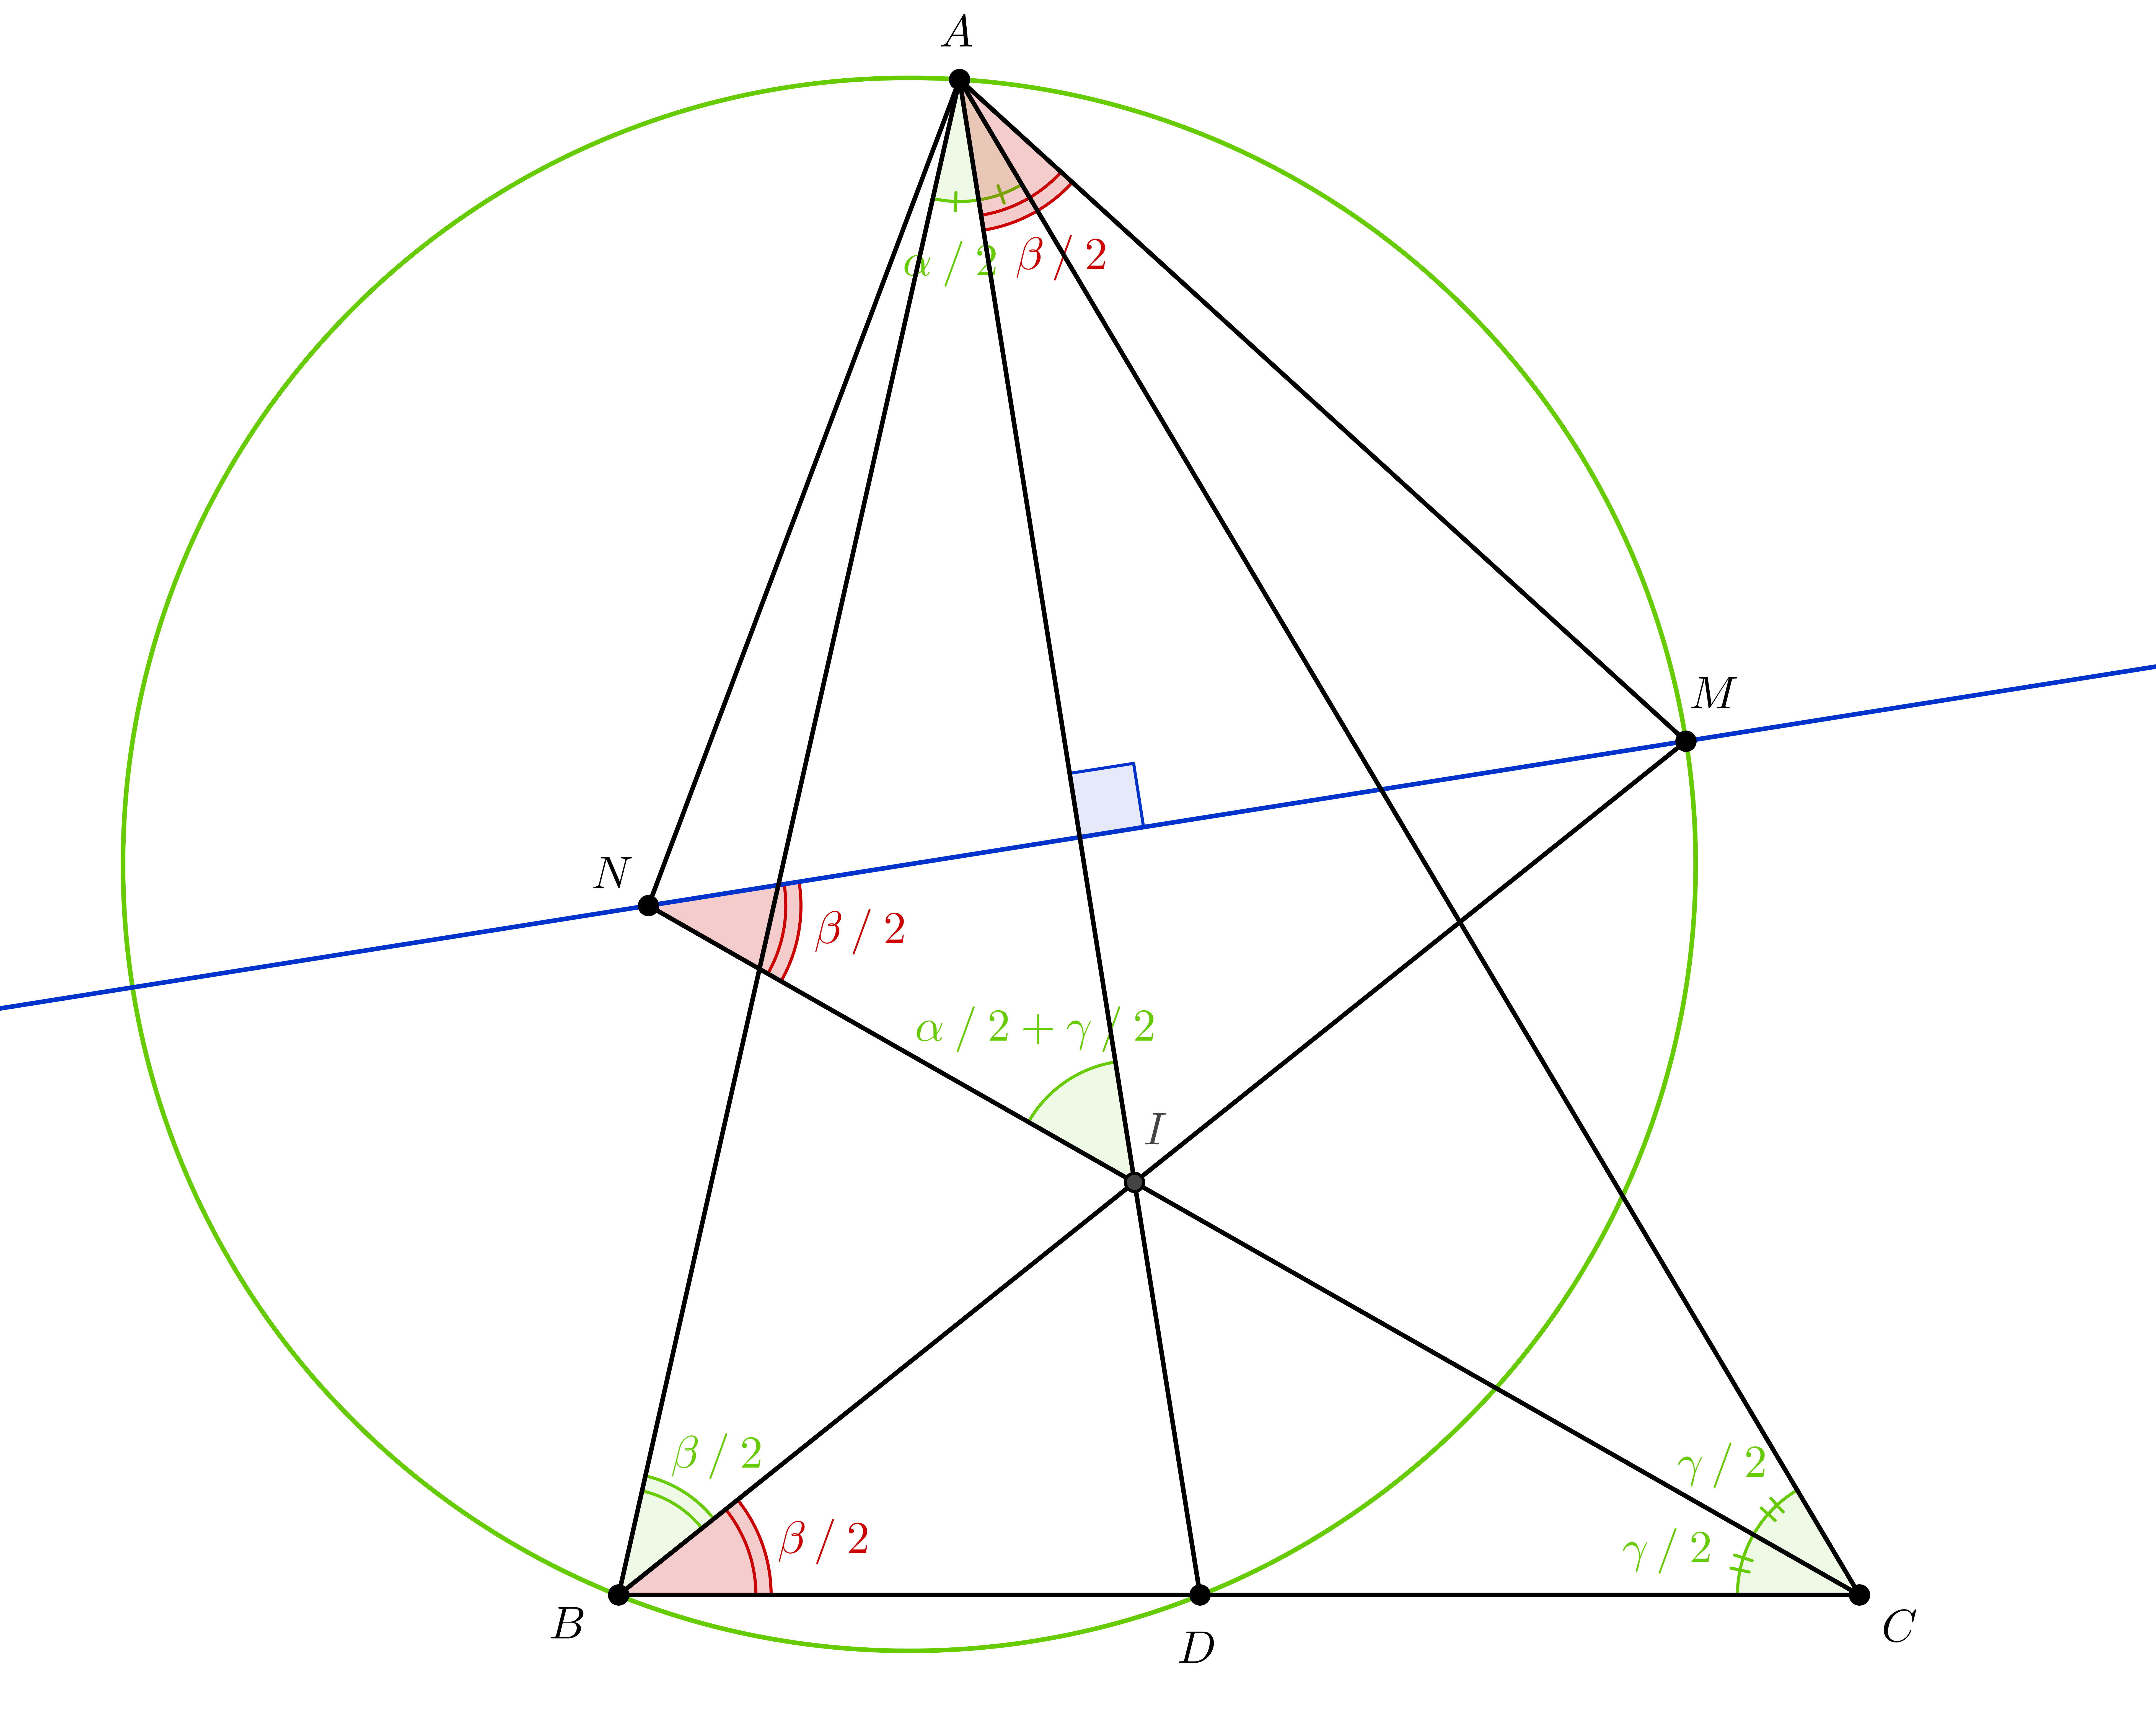
\includegraphics[width=0.75\textwidth]{mediatrice_AD}}
\end{figure}
\end{sol}


\begin{sol}
L'idée ici est de remarquer que la position des points $X$ est contrôlée par le théorème des axes radicaux. En effet, plaçons-nous dans une configuration où les cercles circonscrits aux triangles $AXB$ et $CXD$ sont tangents en un point $X$. On sait alors que la tangente en $X$ et les droites $(AB)$ et $(CD)$ sont concourantes en un point $P$, qui est fixe quelque soit $X$ puisque les points $A$, $B$, $C$ et $D$ sont eux-mêmes fixés. On a alors $PA.PB = PC.PD = PX^2$. Ainsi, pour tout point $X$ appartenant à l'ensemble des points cherchés, la quantité $PX^2$ est constante, ce qui signifie que le lieu des points $X$ ainsi formés est un cercle de centre $P$ et de rayon $\sqrt{PA.PB}$.

\begin{figure}[!h]
\centerline{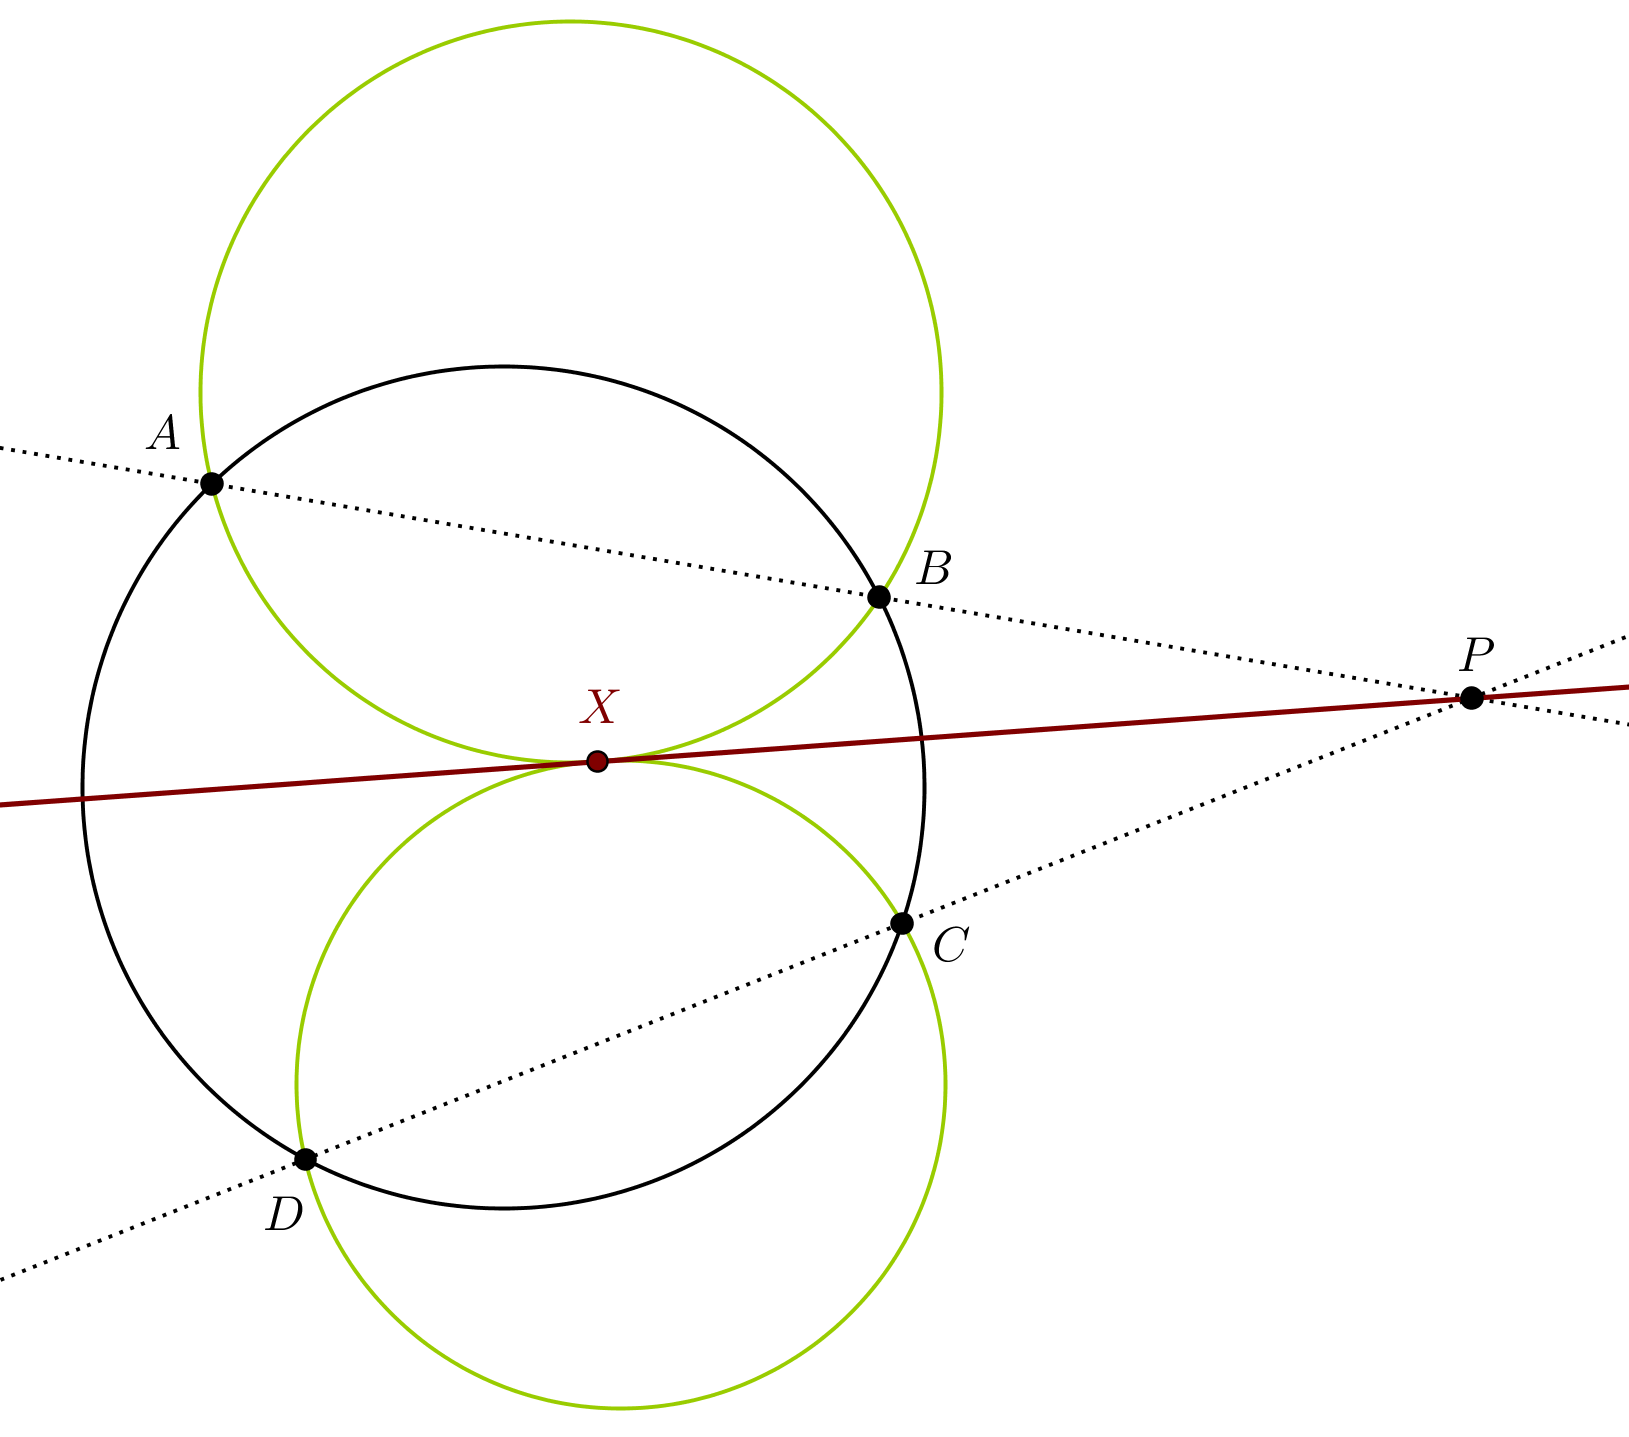
\includegraphics[width=0.55\textwidth]{lieu}}
\end{figure}
\end{sol}